\section{Sistema B – Controlo de Climatização}

Para facilidade de teste, o intervalo de temperaturas é ajustado consoante necessário.\\

\begin{figure}[H]
    \centering
    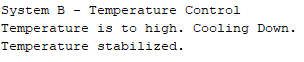
\includegraphics{images/testes/sisB_serialmonitor.png}
    \selectlanguage{portuguese}\caption{Serial Monitor}
\end{figure}
\textbf{Temperature is to high. Cooling Down.}\\
Temperatura ultrapassou máximo definido.\\
\textbf{Temperature stabilized.}\\
Temperatura alcançou mínimo definido.

\begin{figure}[H]
    \centering
    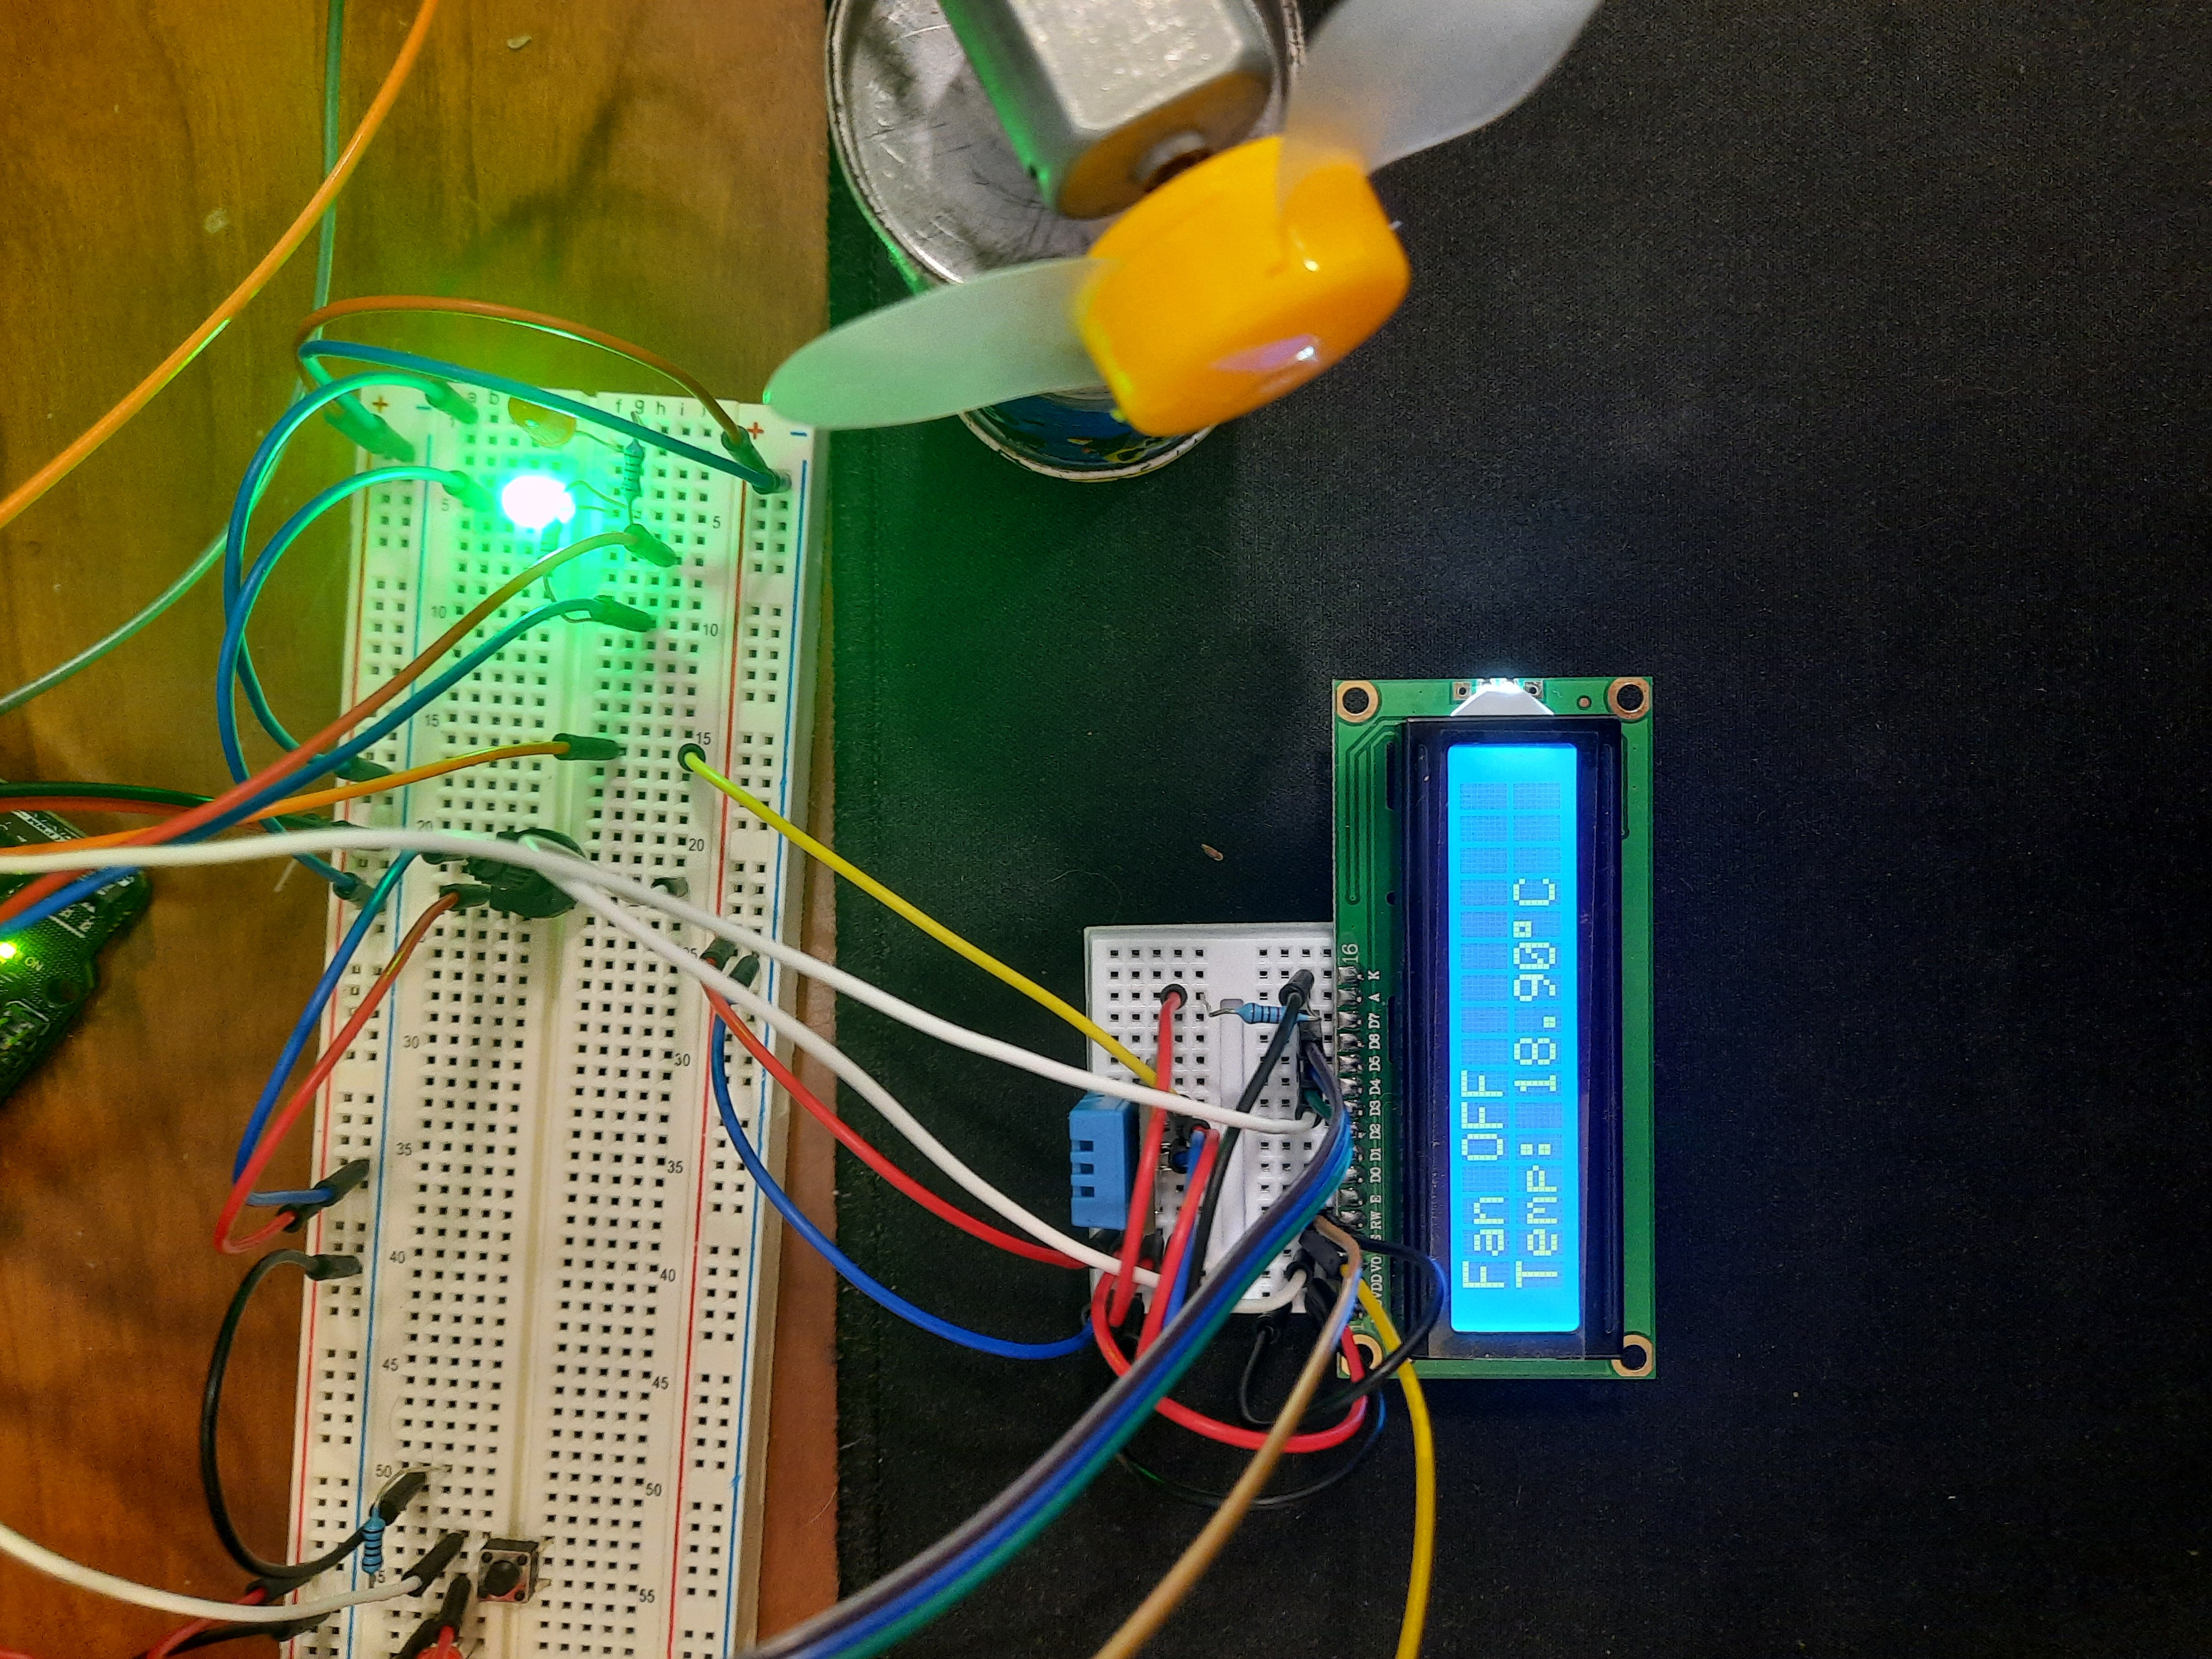
\includegraphics[scale=0.05,angle=-90]{images/testes/sisB_on.jpg}
    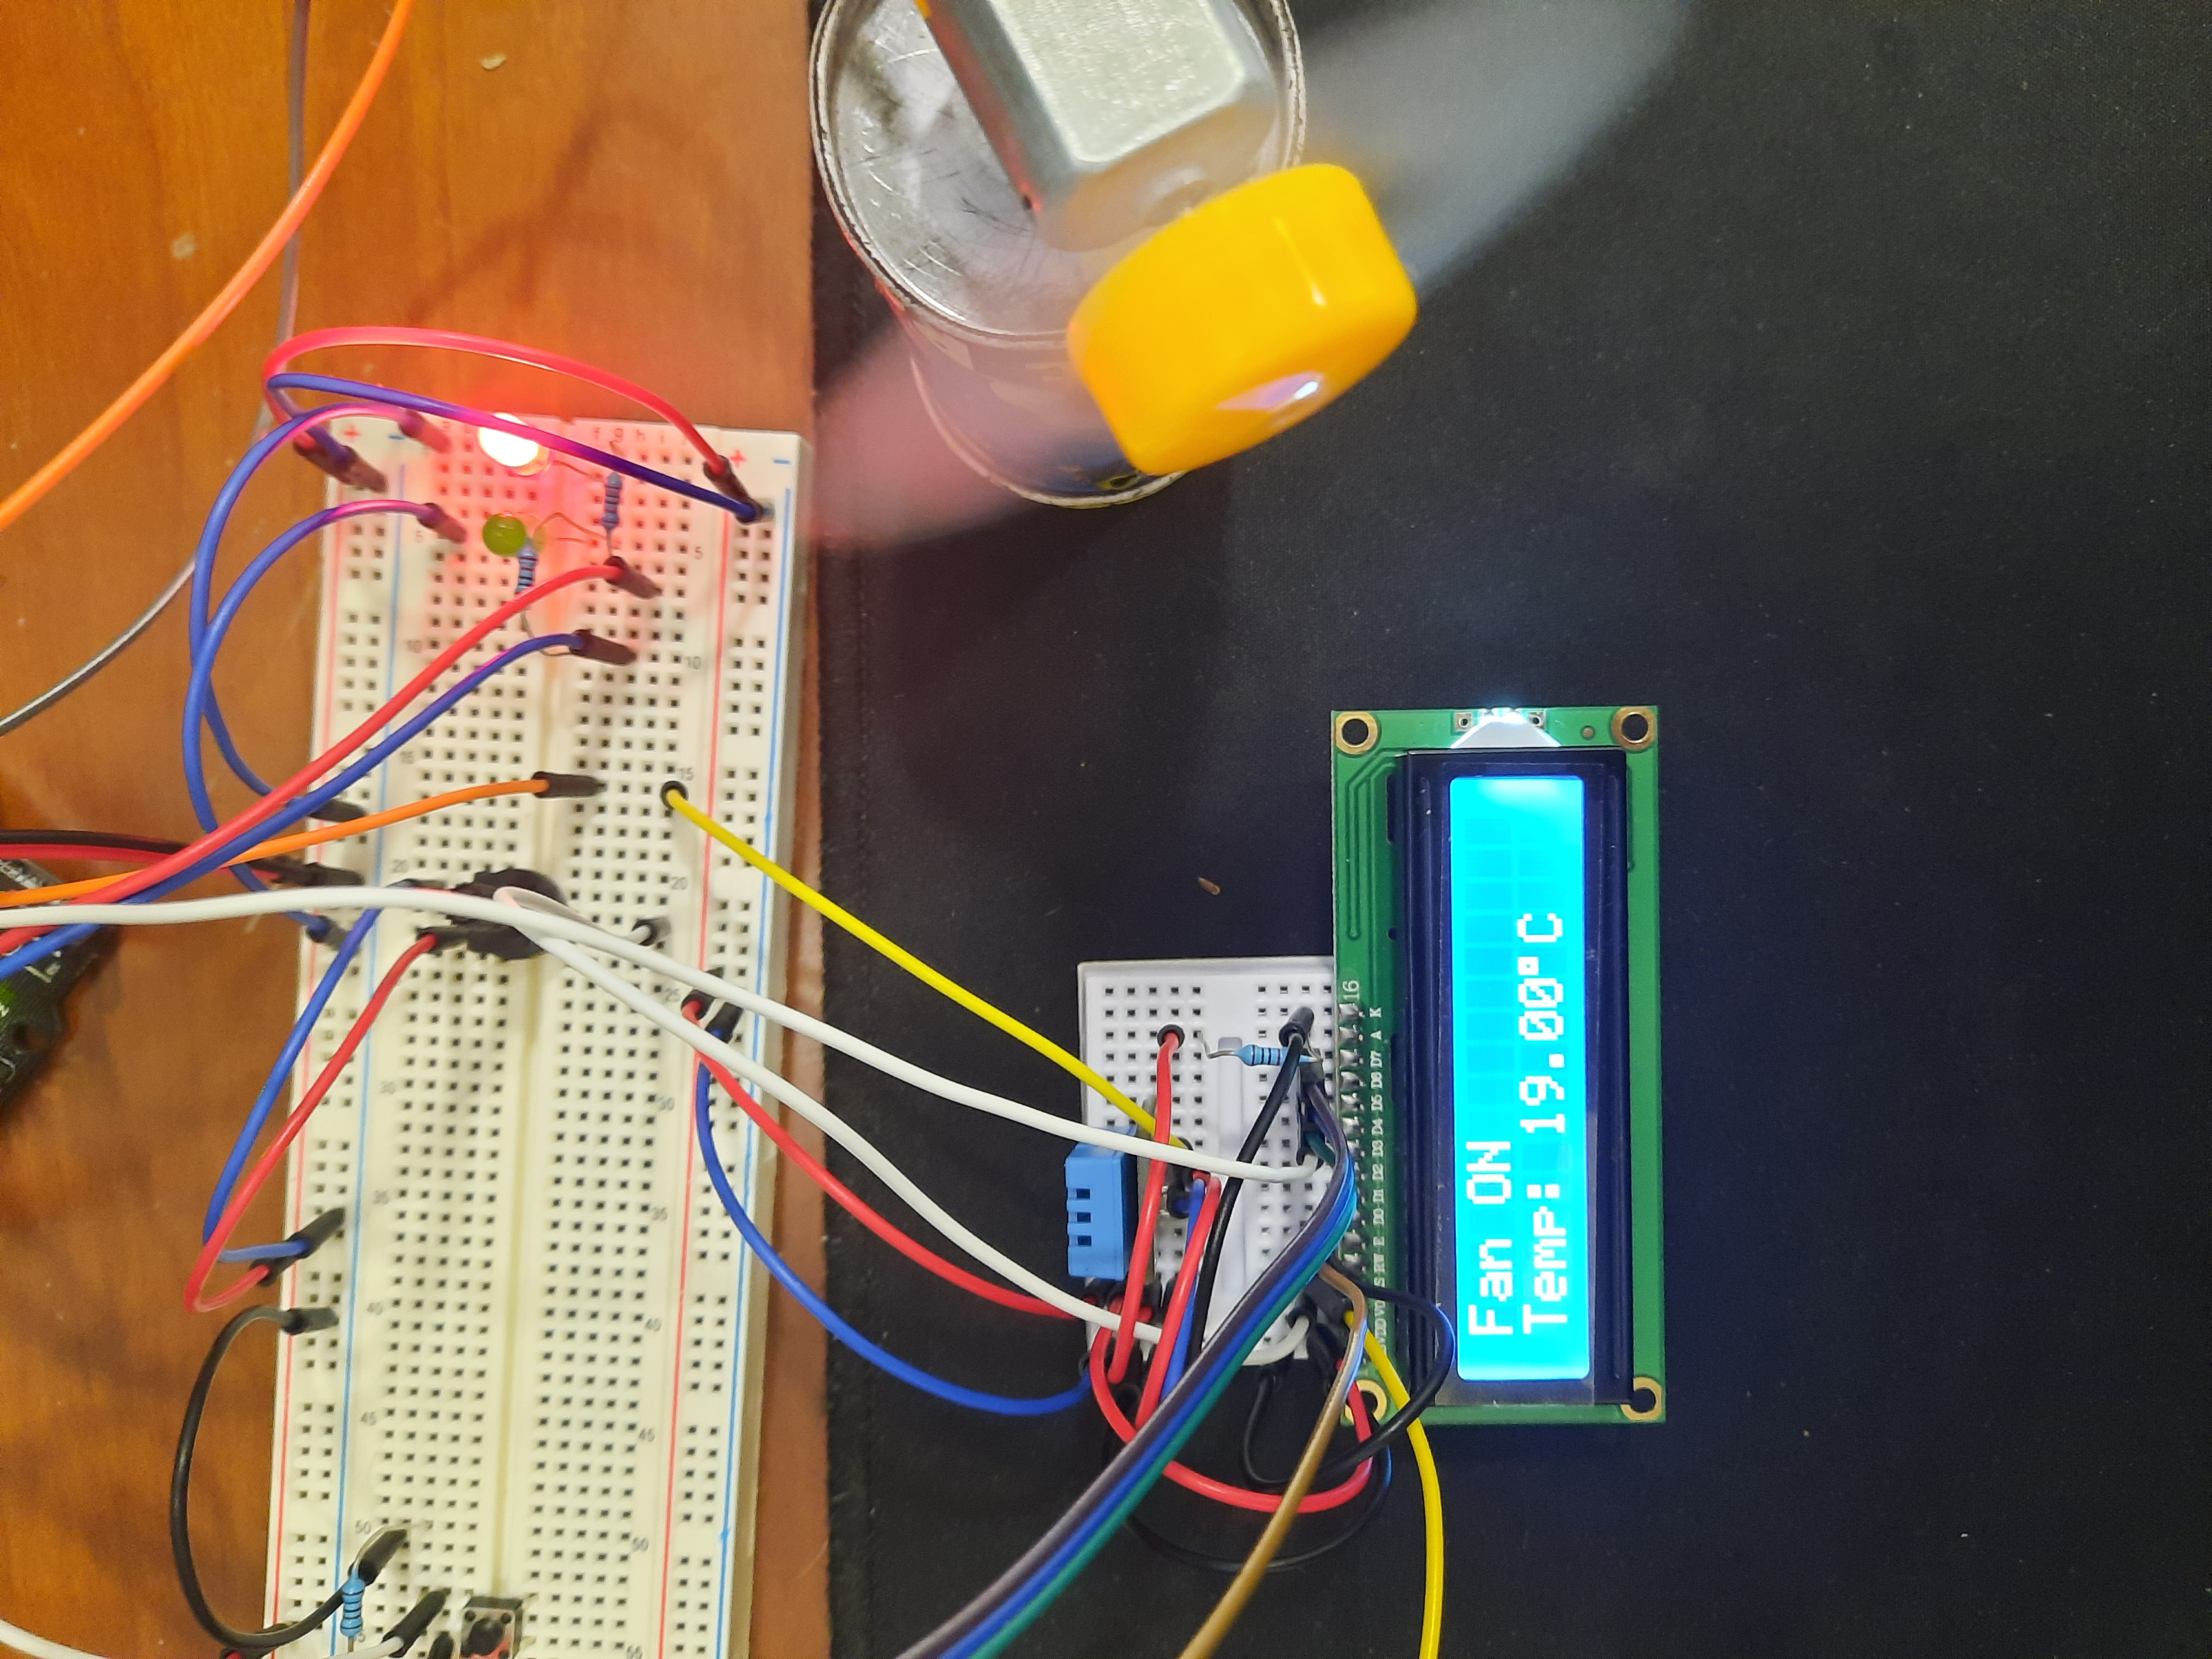
\includegraphics[scale=0.05,angle=-90]{images/testes/sisB_off.jpg}
    \selectlanguage{portuguese}\caption{Stabilized vs Cooling Down}
\end{figure}
